\documentclass[12pt,twoside]{report}
\usepackage[a4paper,width=150mm,top=25mm,bottom=25mm]{geometry}
\usepackage[utf8]{inputenc}
\usepackage{graphicx}\graphicspath{ {images/} }
\usepackage{verbatim}
\usepackage{etoolbox}
\usepackage{tabularx}
\usepackage[hyphens]{url}
\urlstyle{same}
\usepackage{amsmath,amssymb}
\usepackage{amsfonts}
\usepackage{hyperref}
 % \usepackage{dsfont}
\usepackage{rotating}
\usepackage{dcolumn}
\usepackage[export]{adjustbox}
\usepackage{fancyhdr}
\usepackage{csquotes}
\usepackage{multicol}
\usepackage{lipsum}
\usepackage{float}
\usepackage{subcaption}
\usepackage[toc,page]{appendix}
\usepackage{pdfpages}
\pagestyle{fancy}
\renewcommand{\headrulewidth}{0.4pt}
\renewcommand{\footrulewidth}{0.4pt}
\usepackage{caption}
\usepackage[american]{babel}
\usepackage{natbib}
\usepackage[backend=bibtex,style=ieee,natbib=true]{biblatex}
%
\bibliography{chapters/references}
% \bibliography{references}

\usepackage[T1]{fontenc}
\usepackage{titlesec, blindtext, color}
\definecolor{gray75}{gray}{0.75}
\newcommand{\hsp}{\hspace{20pt}}
\titleformat{\chapter}[hang]{\Huge\bfseries}{\thechapter\hsp\textcolor{gray75}{|}\hsp}{0pt}{\Huge\bfseries}

\DeclareMathOperator*{\sumint}{%
\mathchoice%
  {\ooalign{$\displaystyle\sum$\cr\hidewidth$\displaystyle\int$\hidewidth\cr}}
  {\ooalign{\raisebox{.14\height}{\scalebox{.7}{$\textstyle\sum$}}\cr\hidewidth$\textstyle\int$\hidewidth\cr}}
  {\ooalign{\raisebox{.2\height}{\scalebox{.6}{$\scriptstyle\sum$}}\cr$\scriptstyle\int$\cr}}
  {\ooalign{\raisebox{.2\height}{\scalebox{.6}{$\scriptstyle\sum$}}\cr$\scriptstyle\int$\cr}}
}

\fancyhead{}
%\fancyhead[RO,LE]{Thesis Title}
\fancyfoot{}
\fancyfoot[LE,RO]{\thepage}
\fancyfoot[LO,CE]{Chapter \thechapter}
%\fancyfoot[CO,RE]{Tim Ebert}

\makeatletter
\patchcmd{\@caption}{\csname the#1\endcsname}{\csname fnum@#1\endcsname:}{}{}
\renewcommand*\l@figure{\@dottedtocline{1}{1.5em}{4.5em}} 
% default for 3rd arg: 2.3em
\let\l@table\l@figure % as in article.cls
\makeatother


%define the author
\author{Tim Ebert}
\title{Kritische Exponenten von $\phi^4$ Model C bei endlichen Temperaturen}


\def\@makechapterhead#1{%
  \vspace*{50\p@}% <----------------- Space from top of page to Chapter #
  {\parindent \z@ \raggedright \normalfont
    \ifnum \c@secnumdepth >\m@ne
        \huge\bfseries \@chapapp\space \thechapter% <-- Chapter #
        \par\nobreak
        \vskip 20\p@% <-------------- Space between Chapter # and title
    \fi
    \interlinepenalty\@M
    \Huge \bfseries #1\par\nobreak% <------------------ Chapter title
    \vskip 40\p@% <------------------ Space between chapter title and first paragraph
  }}
\newcommand{\rhoPhi}{\rho_{[\mathbf{\Phi}]}}
\begin{document}

%omits page number
\pagenumbering{gobble}
%generates the title
\begin{titlepage}
    %\drop=0.1\textheight
    \centering
    \vspace*{\baselineskip}
    \Large Justus-Liebig-Universität Giessen\\
    \large Fachbereich 07\\
    Institut für Theoretische Physik\\
    \vskip 1em%
    \rule{\textwidth}{1.6pt}\vspace*{-\baselineskip}\vspace*{2pt}
    \rule{\textwidth}{0.4pt}\\[\baselineskip]
    {\huge Differential Basis Integrale für verbessertes Orbital freies }\\[0.4\baselineskip]
    {\large \textit{English title}}\\
    {\LARGE Utilizing Differential Basis Integrals for Improved Orbital Free Machine Learned DFT and Adaptive basis function for KSDFT}\\[0.2\baselineskip]
    \rule{\textwidth}{0.4pt}\vspace*{-\baselineskip}\vspace{3.2pt}
    \rule{\textwidth}{1.6pt}\\[\baselineskip]
    \scshape
    \LARGE \textbf{Master Thesis}\\\vspace{2.pt}
    {\Large im Fach Physik von}\\\vfill
    \textbf{Tim Ebert}\\\vfill
    {\large eingereicht am}\\\vspace{2.pt}
    \textbf{1.11.2025}\\\vfill
    \large
    \vspace{3.2pt}
    \begin{tabular}{cc}
    Betreuer:& Prof. Dr. Fred Hamprecht\\\vspace*{4pt}
    Zweitgutachter:& Prof. Dr. Andreas Dreuw
    \end{tabular}
\end{titlepage}
\newpage
\thispagestyle{plain}
	\large
	\begin{center}
    \textbf{Zusammenfassung}
\end{center}
\normalsize
Es wurden differenzierbare Basis integrale implementiert die genutzt wurden um orbital free basis sets zu fitten und adaptive minimale Basis Sets zu implementieren. Die fähigkeiten dieser geffittenten basis functionen wurde mit anderen klassischen Basis sets verglichen 
	\vspace{5cm}
\begin{center}
	\large
    \textbf{Abstract}
\end{center}
\normalsize
The LPA truncation of the euclidean functional renormalization group (FRG) was formulated for finite temperatures for a O(N)- model with a heat bath attached. The flow equations for the effective potential and the dissipation constant $\gamma$ were determined. Using numerical simulations, the flow equation was solved. Using the data collected in the simulations the effects of dissipation on the phase transition and the flow of the dissipation constant itself were studied for varying initial parameters.



\newpage
\tableofcontents
%\listoffigures
\chapter{Introduction}
\chapter{Introduction}

Density functional theory (DFT) is a field in physics which is commonly applied in the fields of quantum chemistry,
solid state physics and material sciences. It is based on the Hohenberg-Kohn theorems \cite{hohenberg_inhomogeneous_1964} which state that the ground-state properties of a many-electron system are uniquely determined by its electron density.

Based on these insigths Kohn Sham theory was conceived, which strives to reproduce the ground state
density of a complex many-body quantum mechanical system with a set of non-interacting particles which are govered by the much simpler Kohn Sham equation. The non interacting electrons are represented by so called orbitals $\{\phi_i (\mathbf{r})\}_{i=1,...,n}$, which are pairwise orthogonal and normalized. They combine to form the density of the system $\rho(\mathbf{r}) = || \sum\limits_{i=1}^N \phi_i(\mathbf{r})||^2$.

\begin{align}
    H_{KS}[\rho ]  = T_S [\rho] + V_{eff}[\rho]
\end{align}

Dispite its great success KS-DFT has also some short commings. By using orbitals to describe the system it is bound to computationally scale very poorly to larger system sizes. Its accuracy is also heavily dependent on the choice of the exchange correlation functional which is used to approximate the many body effects of the system and the basis on which the orbitals are defined.

New approaches try to fullfill Hohenberg-Kohn promise of a functional dependendent only on the electron density. These approaches are commonly named the Orbital Free DFT (OFDFT) and while older ones use classical density functionals\cite{oldofdft}, newer ones use machine learning models to approximate the functional.\cite{Roman}\cite{zhang_m-ofdft_2023}.

In both cases well shaped basis sets are neccessary to represent the orbitals of kohn sham or the electron density in OF-DFT. Well optimised basis sets for dft calculation exist for a long time \cite{something} but they mostly use fixed basis functions for every atom type to represent the individual orbitals. In some case adaptive basis functions were used to adapt the local basis function to their local environment \cite{something}. But in these  attemps were mostly complicated by the complex integrals which are nessesary to compute the energy of the system. In this work we introduce differentiable integrals which with the help of machine learning technics and automatic diffentaition are  able to optimize baiss sets in an more effective way than previously employed finite difference methods. These integrals can be used to both optimize the orbtials free as well as the kohn sham basis sets for bath their coefficients as well as their exponents. They can also be used to learn advanced adaptive basis functions which use a graph neural network to adapt the basis functions to their local environment , greatly increasing the accuracy of the dft calculation with very minimal cost.
\newpage
\section{Conventions and Notations}
Here we are going to to summarize the conventions that are being followed in this work.
\subsection{Einstein summation}
In this work we are using Einstein summation notation, which is a compact notation for expressing the sum of products of vectors in a vector space. In this notation, summation is implied whenever two indices appear in a product term, one subscript and one superscript. For example, the sum
\begin{align}
    a_i b^i = \sum_{i=1}^n a_i b^i
\end{align}
is implied by the notation. The summation convention is used in this work for all repeated indices, unless otherwise stated.
\subsection{Integral Notation}\label{integral_notation}
We are using Bra-Ket Notation, which is commonly used in quantum mechanics. For two functions $\phi,\psi:\mathbb{R}^3\rightarrow \mathbb{C}$
\begin{align}
    \langle \phi | \psi\rangle &:= \int \phi(\mathbf r)\psi^\dagger(\mathbf r) d\mathbf r
\end{align}
As we are mostly interested in the ground state, which can be described by purely real functions, we can omit the dagger in the notation.
We also note hartree integrals by round brackets, for example
\begin{align}
    (\phi | \psi) &:= \int \int \frac{\phi(\mathbf r)\psi^\dagger(\mathbf r')}{|\mathbf{r}-\mathbf{r'}|} d\mathbf rd\mathbf {r'}
\end{align}
\subsection{Data visualization}\label{boxplots}
To visualize distributions boxplots can give a good overview over the underlying statistics without overcrowding the plotwith to many information. The following visual guide demonstates how the plots used in the work are ment to be interpreted.
\begin{figure}[H]
    \centering
    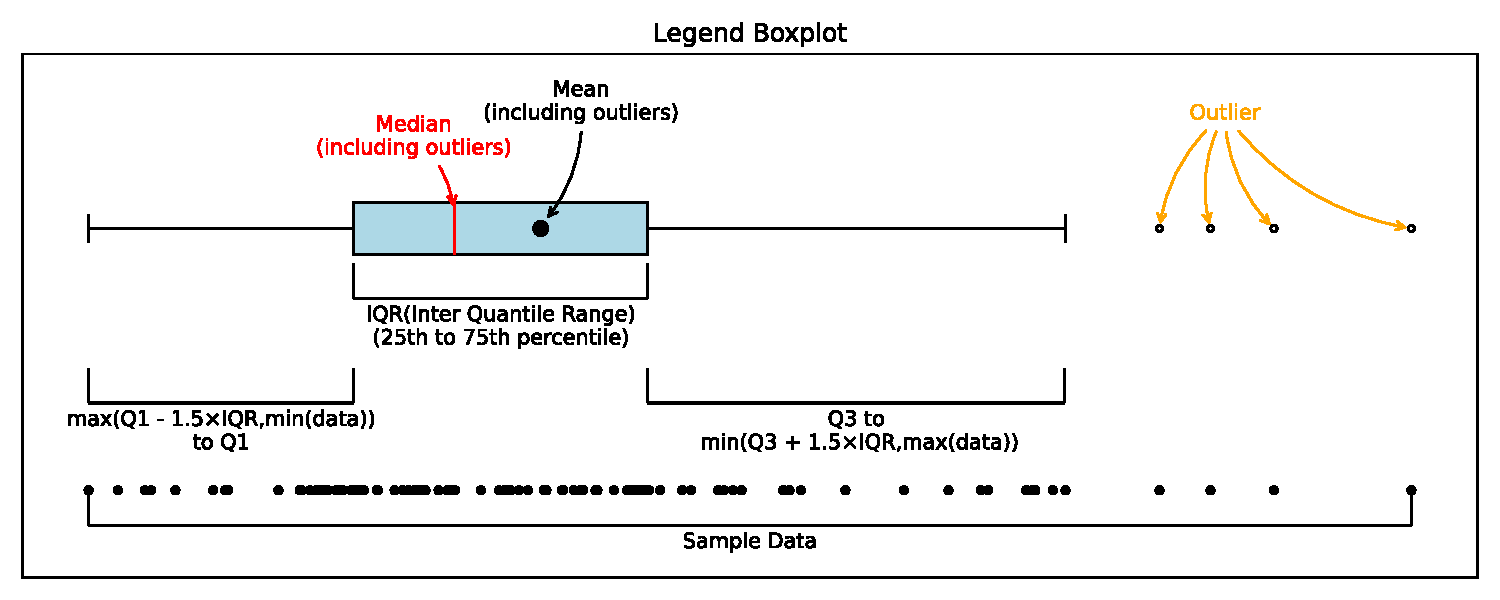
\includegraphics[width=1.\textwidth]{chapters/foundations/images_foundation/legend_boxplot}
    \caption{A boxplot showing the distribution of a toy data set with the important features labeled. Note that the left whiskers is shorted, which indicates that the data is right skewed.}
\end{figure}
Another challenge is the visualisation of the electron density of a molecule. In this work we are
\chapter{Theoretical Foundations}
This section introduces the fundamentals that are neccesary to understand the following chapters. The section is divided into four parts. First the Density functional theory is introduced, followed by the orbital free DFT formulation. The third part introduces the basis sets that are used in DFT calculations. The last part introduces machine learning and the graphformer model that is used in this thesis.




Methods:
Density functional theory and speciffically kohn sham
Basis sets GTOs and PAOs and their integrals. typical basis sets
Orbital free dft formulation basis sets even tempered, density fitting 
Machine learing
Graphformer  Message passing Graph neural network

\section{Density functional theory}
\subsection{Historical Background}
Kohn-Sham Density Functional Theory (KSDFT) stands as a cornerstone in computational quantum mechanics, revolutionizing our approach to electronic structure calculations. Developed by Walter Kohn and Lu Jeu Sham in 1965 \cite{KohnSham1965}, KSDFT extends the foundational work of Hohenberg and Kohn \cite{HohenbergKohn1964} on Density Functional Theory (DFT).
\subsection{Theoretical Foundation}
The theoretical underpinning of DFT rests on two fundamental theorems proved by Hohenberg and Kohn:
\begin{theorem}
The ground-state properties of a many-electron system are uniquely determined by the electron density $n(\mathbf{r})$.
\end{theorem}
\begin{theorem}
There exists a universal functional of the electron density, $F[n(\mathbf{r})]$, which can be used to find the ground-state energy of the system.
\end{theorem}
These theorems establish that the ground-state energy of a system can be expressed as a functional of the electron density:
\begin{equation}
E[n] = F[n] + \int V_{\text{ext}}(\mathbf{r})n(\mathbf{r})d\mathbf{r}
\end{equation}
where $V_{\text{ext}}(\mathbf{r})$ is the external potential and $F[n]$ is a universal functional independent of the external potential.
\subsection{The Kohn-Sham Approach}
Kohn and Sham proposed a practical approach to apply DFT by introducing a fictitious system of non-interacting particles that generate the same density as the system of interacting particles. This approach involves solving a set of single-particle Schrödinger-like equations, known as the Kohn-Sham equations:
\begin{equation}
\left[-\frac{1}{2}\nabla^2 + V_{\text{eff}}(\mathbf{r})\right]\phi_i(\mathbf{r}) = \epsilon_i\phi_i(\mathbf{r})
\end{equation}
where $\phi_i(\mathbf{r})$ are the Kohn-Sham orbitals and $\epsilon_i$ are their corresponding energies. The effective potential $V_{\text{eff}}(\mathbf{r})$ is defined as:
\begin{equation}
V_{\text{eff}}(\mathbf{r}) = V_{\text{ext}}(\mathbf{r}) + V_{\text{H}}(\mathbf{r}) + V_{\text{xc}}(\mathbf{r})
\end{equation}
Here, $V_{\text{ext}}(\mathbf{r})$ is the external potential, $V_{\text{H}}(\mathbf{r})$ is the Hartree potential, and $V_{\text{xc}}(\mathbf{r})$ is the exchange-correlation potential.
\subsection{Contributions to the Kohn-Sham Energy}
The total energy in the Kohn-Sham formulation can be expressed as:
\begin{equation}
E_{\text{KS}} = T_s[n] + E_{\text{H}}[n] + E_{\text{xc}}[n] + E_{\text{ext}}[n]
\end{equation}
Let us examine each term in detail:
\subsubsection{Kinetic Energy of Non-interacting Electrons}
The kinetic energy of the non-interacting electrons, $T_s[n]$, is given by:
\begin{equation}
T_s[n] = -\frac{1}{2}\sum_i \int \phi_i^*(\mathbf{r})\nabla^2\phi_i(\mathbf{r})d\mathbf{r}
\end{equation}
This term represents the kinetic energy of the Kohn-Sham orbitals.
\subsubsection{Hartree Energy}
The Hartree energy, $E_{\text{H}}[n]$, represents the classical electrostatic interaction energy of the electron density:
\begin{equation}
E_{\text{H}}[n] = \frac{1}{2}\int\int \frac{n(\mathbf{r})n(\mathbf{r'})}{|\mathbf{r}-\mathbf{r'}|}d\mathbf{r}d\mathbf{r'}
\end{equation}
\subsubsection{Exchange-Correlation Energy}
The exchange-correlation energy, $E_{\text{xc}}[n]$, encapsulates all many-body effects beyond the Hartree approximation. Its exact form is unknown, and developing accurate approximations for this term is a central challenge in DFT. Common approximations include:
\begin{itemize}
\item Local Density Approximation (LDA):
\begin{equation}
E_{\text{xc}}^{\text{LDA}}[n] = \int n(\mathbf{r})\epsilon_{\text{xc}}(n(\mathbf{r}))d\mathbf{r}
\end{equation}
where $\epsilon_{\text{xc}}(n)$ is the exchange-correlation energy per particle of a uniform electron gas of density $n$.
\item Generalized Gradient Approximation (GGA):
\begin{equation}
E_{\text{xc}}^{\text{GGA}}[n] = \int f(n(\mathbf{r}), |\nabla n(\mathbf{r})|)d\mathbf{r}
\end{equation}
where $f$ is a function of both the density and its gradient.
\end{itemize}
\subsection{External Potential Energy}
The external potential energy, $E_{\text{ext}}[n]$, represents the interaction of the electrons with the external potential (typically due to the nuclei):
\begin{equation}
E_{\text{ext}}[n] = \int V_{\text{ext}}(\mathbf{r})n(\mathbf{r})d\mathbf{r}
\end{equation}
\section{Self-Consistent Field Method}
The Kohn-Sham equations are solved iteratively using the Self-Consistent Field (SCF) method:
\begin{enumerate}
\item Start with an initial guess for $n(\mathbf{r})$
\item Calculate $V_{\text{eff}}(\mathbf{r})$
\item Solve the Kohn-Sham equations to obtain $\phi_i(\mathbf{r})$
\item Calculate a new density: $n_{\text{new}}(\mathbf{r}) = \sum_i |\phi_i(\mathbf{r})|^2$
\item If $|n_{\text{new}}(\mathbf{r}) - n(\mathbf{r})| < \text{tolerance}$, stop. Otherwise, return to step 2 with $n(\mathbf{r}) = n_{\text{new}}(\mathbf{r})$
\end{enumerate}

\section{Orbital free DFT}
Rooted in the original formulation of Density Functional Theory by Hohenberg and Kohn \cite{HohenbergKohn1964}, Orbital-Free Density Functional Theory (OF-DFT) aims to calculate the ground state properties of a many-electron system directly from the electron density, without the need for individual electronic orbitals.
\subsection{Theoretical Foundation}

Based on equation \eqref{eq:energy_density} the total energy of a system can be expressed as a functional of the electron density $\rho(\mathbf{r})$. The challenge of Orbtial free DFT lies in finding an accurate representation of the kinetic energy functional from equation \eqref{eq:kin} directly from the density, without resorting to orbitals. Historic attemps\cite{thakkar1992comparison,wang1999orbital} at this used numerical approximations. Known approximation include the Thomas-Fermi functional\cite{thomas_fermi_1927} and the von Weizsäcker functional\cite{von_weizsacker_1935}. These functionals were based on the kinetic energy of a non-interacting electron gas and its gradient.
\subsubsection{Thomas-Fermi Functional}
The simplest approximation is the Thomas-Fermi functional:
\begin{equation}
T_{TF}[n] = C_{TF} \int n^{5/3}(\mathbf{r}) d\mathbf{r}
\end{equation}
where $C_{TF} = \frac{3}{10}(3\pi^2)^{2/3}$.
\subsubsection{von Weizsäcker Functional}
The von Weizsäcker functional then adds a additional gradient correction:
\begin{equation}
T_{vW}[n] = \frac{1}{8} \int \frac{|\nabla n(\mathbf{r})|^2}{n(\mathbf{r})} d\mathbf{r}
\end{equation}
\subsubsection{Generalized Gradient Approximation (GGA)}
More sophisticated functionals incorporate higher-order density gradients:
\begin{equation}
T_{GGA}[n] = \int t_{GGA}(n(\mathbf{r}), \nabla n(\mathbf{r}), \nabla^2 n(\mathbf{r}), ...) d\mathbf{r}
\end{equation}

If one can represent the total energy of the system as a function of density, the ground state can be found by minimizing the total energy functional using conventional techniques like gradient descent. With the rise of machine learning in DFT, a promising approach is to learn an empirical approximation of the kinetic energy functional from a large dataset of electronic structure calculations.
While initial attempts by Remme et al. and Imoto et al. \cite{remme_kineticnet_2023,imoto2021order} used grid-based density representations, \textsc{M-OFDFT} \cite{zhang_m-ofdft_2023} pioneered the use of atom-centered basis functions, achieving the first successful prediction of energies with chemical accuracy across a large set of geometries. \textsc{M-OFDFT} also introduced the use of individual Self-Consistent Field (SCF) algorithm steps to generate model labels.
However, these labels were insufficient for the model to emulate the true functional around the ground state accurately enough to allow convergence of the minimization procedure. Instead, the density coefficients tended to drift in unphysical directions, necessitating a complicated halting criterion to generate densities near the ground state.
\subsection{OF-DFT label generation}\label{ofdft_labelgen}
In the following, we will describe the label generation process proposed by the authors of M-OFDFT \cite{zhang_m-ofdft_2023} and the modifications we made to increase training data diversity and improve model convergence.\\
In the following we will use the following conventions:\\
We denote the orbital basis functions as $\{\eta_\mu(\mathbf{r})\}_{\mu=1,...,N_\text{basis}}$, which when contracted with the coefficients $\{C_{i,\mu}\}_{i=1,..,N_\text{electrons},\mu=1,...,N_\text{basis}}$ describe the orbitals $\phi_i(\mathbf{r}) = C_i^\mu \eta_\mu(\mathbf{r})$. The orbitals can be used to calculate the electron density $\rho(\mathbf{r}) = \sum_{i=1}^{N_\text{electrons}}\phi_i(\mathbf{r})^2=\sum_{i=1}^{N_\text{electrons}}C_i^\mu \eta_\mu(\mathbf{r})C_i^\nu \eta_\nu(\mathbf{r}) =  \eta_\mu(\mathbf{r})\Gamma^{\mu,\nu} \eta_\nu(\mathbf{r})$. Where we defined the density matrix $\Gamma^{\mu,\nu} = \sum_{i=1}^{N_\text{electrons}}C_i^\mu C_i^\nu$.\\
To describe the density in the orbital free basis we use another basis set $\{\omega_\mu(\mathbf{r})\}_{\mu=1,...,N_\text{of-basis}}$ with corresponding coefficients $\mathbf{p} =\{p^\mu\}_{\mu=1,...,N_\text{of-basis}}$ which form a linear basis for the density $\rho_\text{OF}(\mathbf{r}) = p^\mu \omega_\mu(\mathbf{r})$.\\
We also use the follwing symbols to denote common basis integrals between the two basis sets following the conventions introduced in section \ref{integral_notation}:
\begin{align}
    W_{\mu\nu} &= \langle\omega_\mu |\omega_\nu\rangle\\
    L_{\mu,\nu\gamma} &= \langle \omega_\mu |\eta_\nu\eta_\gamma\rangle\\
    D_{\alpha,\beta,\gamma,\delta}  &= \langle\eta_\alpha\eta_\beta|\eta_\gamma\eta_\delta\rangle\\
    \tilde{W}_{\mu\nu} &= (\omega_\mu |\omega_\nu)\\
    \tilde{L}_{\mu,\nu\gamma} &= (\omega_\mu |\eta_\nu\eta_\gamma)\\
    \tilde{D}_{\alpha,\beta,\gamma,\delta}  &= (\eta_\alpha\eta_\beta|\eta_\gamma\eta_\delta)\\
    S_{\alpha,\beta} &= \langle \eta_\alpha|\eta_\beta\rangle\\
    {v_{ext}}_\mu &= \int \omega_\mu (r) V_{ext} (r)dr\\
    {V_{ext}}_{\mu,\nu} &= \langle \eta_\mu | V_{ext} (r) | \eta_\nu \rangle
\end{align}
We are now set to describe the label generation process.\\
\subsubsection{Density fitting}\label{into_density_fitting}
Density fitting is a procedure to represent the density produced by the Kohn-Sham orbitals using orbital-free basis functions $\{\omega_\mu(\mathbf{r})\}_\textit{\mu=1,...,N_\text{of-basis}}$, while preserving its electronic properties. This mean calculating $\mathbf{p}(\{C_{i,\mu}\}_{i=1,..,N_\text{electrons},\mu=1,...,N_\text{basis}})$.\\
In chapter \ref{chapter:densityfitting}, we define and evaluate different density fitting algorithms and compare the properties of the densities they produce.\\
\subsubsection{Energy and gradient label generation}
The label for the kinetic energy in coordinates is indirectly calculated by:

\begin{align}
    T_S(\mathbf{p}) = T_S(C) + E_{H}(C) + E_{XC}(C) + E_{ext}(C) - E_{H}(\mathbf{p}) + E_{XC}(\mathbf{p}) + E_{ext}(\mathbf{p}).
\end{align}

We cannot calculate the gradient of the kinetic energy directly from this equation as the orbital free density coefficients $\mathbf{p}$ are dependent on
the coefficients in the orbital basis $\{C_{i,\mu}\}_{i=1,..,N_\text{electrons},\mu=1,...,N_\text{basis}}$ in a nontrivial way.\\
Instead, we make use of the minimization procedure in the KSDFT calculation. Additionally we use a method developed by Manuel Klockow which in each iteration of the self consistent field procedere adds an additional pertubation to the effective potential to increase the diversity of the densities in the labels. In each iteration the next set of orbitals is then computed as follows:

\begin{align}
    \Phi^{k} = \underset{\{\phi_i\}_{i=1}^n \text{orthonormal}}{\text{argmin}} \langle \psi_{\mathbf{\phi}} | \hat T_S | \psi_{\mathbf{\phi}} \rangle + \sum_{k'<k} \pi^{(k')}_k V_{eff}^{k'}[\rho_{[\mathbf{\phi}]}] + V_\text{peturb}^{k}(\rhoPhi)
\end{align}


Where $\pi^{(i)}_k$ are the DIIS coefficients of the KSDFT calculation and

\begin{align}
    V_{eff}^{k'}[\rho_{[\mathbf{\phi}]}] = \int \rho_{[\mathbf{\phi}]}(\mathbf{r}) V_{eff[\rho_{[\mathbf{\phi}^{k'}]}]}(r)dr\\
    V_\text{peturb}^{k}(\rhoPhi) = \int \rhoPhi(\mathbf{r}) v_{\text{peturb},\mu}^{k}\omega_\mu(\mathbf{r})dr
\end{align}
is the effective potential of the $k'$-th iteration integrated over the density of the new density and the pertubation of the effective potential of the $k$th iteration. With $v_{\text{peturb},\mu}^{k} \sim \epsilon_k * \mathcal{N}(1,0)$ and $\omega_\mu$ being basis function in the orbital free basis.
$\epsilon_k$ is then chosen such that starts at the 5 interation and decreases over time.
This is solved using Laplace multipliers:

\begin{align}
    \frac{\delta T_S[\rho_{[\mathbf{\phi}^{k}]}]}{\delta \rho}(\mathbf{r}) + \sum_{k'<k} \pi^{(k')}_k V_{eff}^{k'}(\mathbf{r}) + v_{\text{peturb},\mu}^{k}\omega_\mu(\mathbf{r})= \mu^{(k)}
\end{align}
From here we cannot compute the gradient of the kinetic energy exactly but we can calculate its projection in the plane of constant particle numbers. As in density optimisation our searchspace is restricted to this plane this is sufficient for our purposes.
The projected gradient of the kinetic energy is then calculated as the DIIS weighted average over the projected last few effective potentials:

\begin{align}
    \nabla_\mathbf{p} T_S(\mathbf{p}) &= \int \frac{\delta T_S[\rho_{[\mathbf{\phi}^{k}]}]}{\delta \rho}(\mathbf{r}) \mathbf{\omega}(\mathbf{r}) d\mathbf{r} \\
    &= -\int\sum_{k'<k} \pi^{(k')}_k V_{eff}^{k'}(\mathbf{r}) \mathbf{\omega}v_{peturb,\mu}^{k}\omega_\mu(\mathbf{r})(\mathbf{r}) +\mu^{(k)}\mathbf{\omega}(\mathbf{r})d\mathbf{r} = -{\mathbf{v}}_{eff\{\mathbf{p}^{k'}\}_{k'< k}}+\mu^{(k)}\mathbf{w}\\
    \left( \textbf{I}-\frac{\textbf{w}^{(d)}{\textbf{w}^{(d)}}^T}{{\textbf{w}^{(d)}}^T
        \textbf{w}^{(d)}}\right) \nabla_\mathbf{p} T_S(\mathbf{p}) &= -\left( \textbf{I}-\frac{\textbf{w}^{(d)}{\textbf{w}^{(d)}}^T}{{\textbf{w}^{(d)}}^T
        \textbf{w}^{(d)}}\right){\mathbf{v}}_{eff\{\mathbf{p}^{k'}\}_{k'< k}}\\
    \mathbf{v}_{eff}(\mathbf{p}) &= \nabla_\mathbf{p} (E_{H}(\mathbf{p}) + E_{XC}(\mathbf{p}) + E_{ext}(\mathbf{p}))
\end{align}
These labels for the kinetic energy are then used to train a machine learning model to emulate the kinetic energy functional.\\

\subsection{Preparation of the data}
To prepare the data for machine learning, we employ the same techniques as in the original M-OFDFT \cite{zhang_m-ofdft_2023} paper. We briefly describe their functions here.
\subsubsection{Natrep}
Orthogonalizing the orbital-free basis for more meaningful coefficients.
\subsubsection{Dimensionwise rescaling}
Statistics are calculated for the coefficients of each atom type in the dataset, and the coefficients are rescaled to have a mean of 0 and a standard deviation of 1.
\subsubsection{Local frames}
To make the model rotationally invariant, a local coordinate system is defined for each atom, oriented towards its nearest neighbor. The coefficients are then projected into this local frame.

\section{Basis sets}
In order to represent spacial functions $f:\mathbb{R}^3\right \mathbb{C}$ inside a DFT calculation atom centric basis sets are most commonly used, as they provide anhanced resolution around the nuleii where most of the electron density is concentrated.
\subsection{Contracted atomic orbitals}
Contracted atomic orbitals are defined as a linear combination of a larger primary basis of basis functions centered on atom centers. Formally we can write a contracted atomic orbitals basis function $\eta_{\mu}(\mathbf{r})$ as a weighted sum of the primary basis functions $\tilde\eta_\nu(\mathbf{r})$ where $\mu,\nu$ are belonging to the same Atom.
\begin{align}
    \eta_{\mu} &=\sum\limits_{\nu} A_{\mu,\nu} \tilde \eta_{\nu}
\end{align}
\subsection{Contracted Gaussian Type Orbitals (CGTOs)}
The radial distribution of primary basis functions $\eta_{\mu}(\mathbf{r})$ is typically chosen as Gaussians centered on the same atom at position $\mathbf{R}$ with different exponents, multiplied by spherical harmonics $Y_{lm}$ to introduce angular dependency.
\begin{align}
\eta_{\mu}(\mathbf{r}) &= N(\alpha,m,l) ||\mathbf{r}-\mathbf{R}||^l Y_{lm}(\frac{\mathbf{r}-\mathbf{R}}{||\mathbf{r}-\mathbf{R}||}) e^{-\alpha ||\mathbf{r}-\mathbf{R}||^2}
\end{align}
where $N(\alpha,m,l)$ are normalisation constants.
Gaussian orbitals offer several advantages: they are computationally efficient, easily integrated, and the product of two Gaussians remains a Gaussian, which simplifies many otherwise complex integrals. However, a single Gaussian cannot accurately describe the electron density cusp near the nucleus. To address this, primitive Gaussians are typically contracted to Contracted Gaussian-Type Orbitals (CGTOs) to form a more physically representative basis set. The contraction coefficients $A_{\mu,\nu}$ are fitted to more accurate basis functions like Slater-type orbitals (STOs).
Spherical harmonics provide arbitrary angular resolution and can be formulated in their Cartesian representation as a polynomial of order $l$.
\begin{align}
    ||\mathbf{v}||^l Y_{lm}(\frac{\mathbf{v}}{||\mathbf{v}||}) &= \sum\limits_{a,b,c\in \mathbb{N}_0 a+b+c\leq l} A_{l,a,b,c} v_1^a v_2^b v_3^c
\end{align}
Where $A_{l,a,b,c}$ are constants. This leads to CGTOs just being finite sums of finite polynominals multiplied with gaussians.

\subsection{Integrals}
Most relevant integrals for DFT involve integrals over products of gaussians which can be computed analytically. Examples are the overlap integral $\langle \eta_{\mu}|\eta_{\nu}\rangle$, the kinetic energy integral $\langle \nabla \eta_{\mu}|\nabla \eta_{\nu}\rangle$, the electron-nucleus integral $\langle \eta_{\mu}|\frac{Z}{||\mathbf{r}-\mathbf{R}||}|\eta_{\nu}\rangle$ as well as the hartree integral $(\eta_{\mu}\eta_{\nu}|\eta_\gamma\eta_\delta)$. While these closed form solutions exist they still involve many repeated recursion relations and can be very compute intensive for larger molecules. Other more complicated integrals, such as the Thomas Fermi functional or the von Weizsäcker functional, as well as practically all exchange correlation functionals, are usually computed numerically on a sufficently large grid. In this work we are using the implementationa of the libcint library \cite{sun_libcint_2015} to compute these integrals, when they don't have to be differentiable.


\section{Machine Learning}
Machine Learning is since .. Nobel price 2024


\section{Graph Neural Networks}
Graph neural networks are a special Variant of Neural networks that apply to graph shaped data.
In our case the graph is the molecular structure of the system that we want to model. Each atom functions as a node in the graph which contains information about the local density around this atom in form of the coefficients of the basis function that centered on the atom. The Edges of the graph contain information in form of the distance towards the next atom. These distances can be embedded in the edge features of the graph neural network.

\subsection{Messagepassing Neural Network}
Message Passing Neural Networks (MPNNs) operate on graph-structured data G = (V, E), where V is the set of nodes and E is the set of edges. The core of MPNNs is the message passing operation, defined as:

\begin{align}
m_t^{(v)} &= \text{AGG}\left(\{M_t(h_t^{(v)}, h_t^{(u)}, e_{vu}) \mid u \in N(v)\}\right) \\
h_{t+1}^{(v)} &= U_t(h_t^{(v)}, m_t^{(v)})
\end{align} 
    

where $h_t^(v)$ is the hidden state of node $v$ at time step $t$, $e_vu$ is the edge feature between nodes $v$ and $u, N(v)$ is the neighborhood of $v, M_t$ is the message function, AGG is an aggregation function (e.g., sum, mean, max), and $U_t$ is the update function. These operations are performed for $T$ time steps to capture higher-order interactions in the graph.

\subsubsection{Embeddings}
The atomic number of every atom is one hot encoded into a vector which length the number of distinct atomtypes in the dataset is. The distance between the atoms Is embedded using besselfunction following the approach of \cite{https://arxiv.org/pdf/2003.03123}. See figure \ref{fig:bessel_embedding}
\begin{align}
    \tilde{e}_{\text{RBF},n}(d) &= \sqrt{\frac{2}{c}}\frac{\sin(\frac{\omega_n }{c})}{d}\hspace{2cm} \omega_n :=(n+1)d\pi\\
    u(d)&= 1-\frac{(p+1)(p+2)}{2}d^p + p(p+2)d^{p+1}-\frac{p(p+1)}{2}d^{p+2}
\end{align}
Where we choose p = 1 and c = 6, as most of the bonds in our dataset are shorter than 6 Angstrom as can be seen in figure \ref{fig:bond_length}. The distance embedding is then multiplied with the one hot encoded atomic number of the atom to get the final edge feature.

\begin{figure}
    \centering
    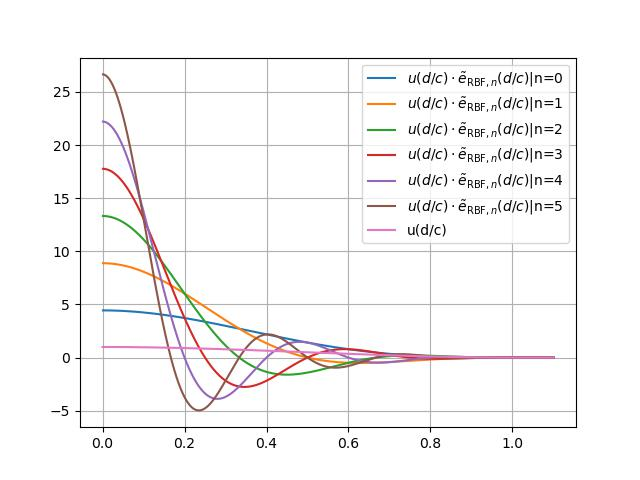
\includegraphics[width=0.8\textwidth]{chapters/foundations/images_foundation/bessel_embedding}
    \caption{The initial basis function used for the distance embedding in the graph neural network.}
    \label{fig:bessel_embedding}
\end{figure}
\begin{figure}
    \centering
    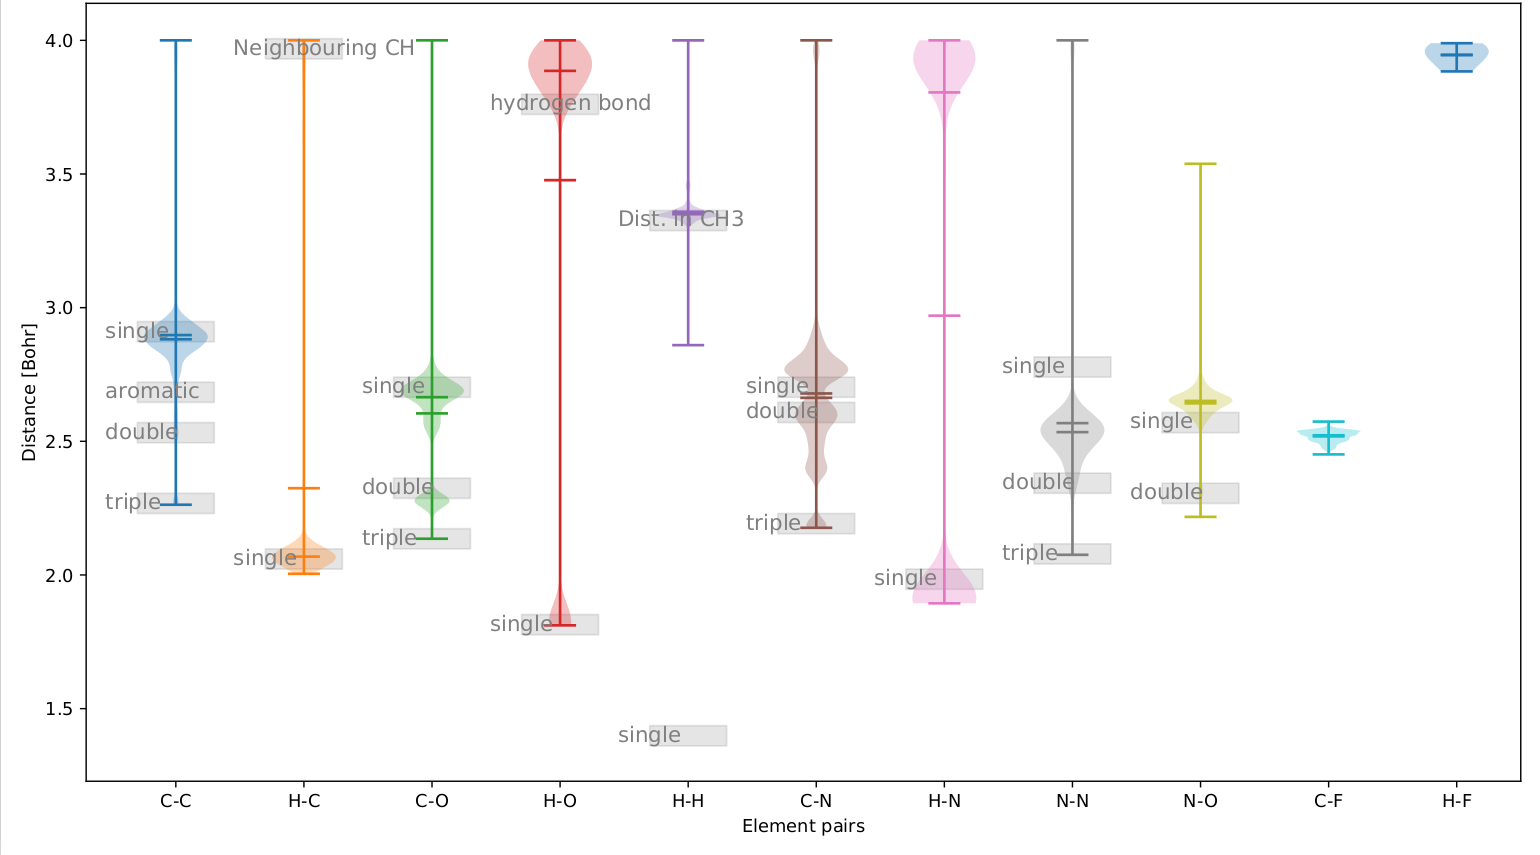
\includegraphics[width=0.8\textwidth]{chapters/foundations/images_foundation/bondlength}
    \caption{The average Bondlength appearing in QM9(Credit Tobias)}
    \label{fig:bond_length}
\end{figure}
For the final embedding of the edge features the one hot encoded atomic number of the incomming and outcomming atom is concatenated with the distance embedding. This is then passed through a short MLP\cite{mlp} with scip connection:
%\begin{align}
%        h_i:= \text{HOTONE(z_i)}\in R^{n_z}\\
%        e_{\text{edge embedding},i,j}^{(0)} = \sigma((h_i||h_j||\text{emb_{ij}})W_{\text{edge}}+b_{\text{edge}})\\
%    e_{\text{edge embedding},i,j}^{(1)} &= u(d_{i,j})(x_{\text{edge embedding}}^{(0)} + \text{MLP}(x_{\text{edge embedding}}^{(0)}))
%\end{align}
These edge features are then aggregated into node features using an aggregation function. The Node features are then futher processed.
\begin{align}
    n_{node_{features},i}^{(0)} &= \text{AGG}(e_{\text{edge embedding},i,j}^{(1)})_i + h_{i}W_{\text{node}} + b_{\text{node}} \\
    n_{node_{features},i}^{(l+1)} &= \text{BatchNorm}(n_{node_{features},i}^{(l)} + \text{MLP}(n_{node_{features},i}^{(l)}))
\end{align}
Then iterativly new edge messages are contructed from these node features and again aggregated to node features:
\begin{align}
    e_{\text{edge embedding},i,j}^{(l+1)} &= \text{MLP}(n_{node_{features}i}^{(l)}||n_{node_{features},j}^{(l)}||e_{\text{edge embedding}i,j}^{(l)})\\
    n_{node_{features},i}^{(l+1)} &= \text{AGG}(e_{\text{edge embedding},i,j}^{(l+1)})_i + n_{node_{features},i}^{(l)}
\end{align}
\subsection{Graphformer}
The architecture for the much more expressive model used for OFDFT is the Graphformer. The Graphformer is a transformer like architecture that operates on graph structured data, in this case a complete graph but takes into account the distances between different nodes in its attention module. \cite{Graphformer}.
We also intotroduce a Atomic reference module as it was done in Mofdft\cite{zhang_m-ofdft_2023}.

\begin{appendices}
\end{appendices}
\printbibliography[heading=bibintoc, title={Complete bibliography}]
%Displays the whole bibliography with the title "Complete bibliography"                  
\clearpage
%Filtering bibliography
\newpage
%\includepdf[pages=1]{images/Selbststaendigkeitserklaerung.pdf}

\end{document}